\begin{frame}{Scaling}
    \begin{itemize}
        \item Use when different numeric features have different scales (different range of values)
        \begin{itemize}
            \item Features with much higher values may overpower the others
        \end{itemize}
        \item Goal: bring them all within the same range
        \item Different methods exist
    \end{itemize}

    \begin{figure}
        \centering
        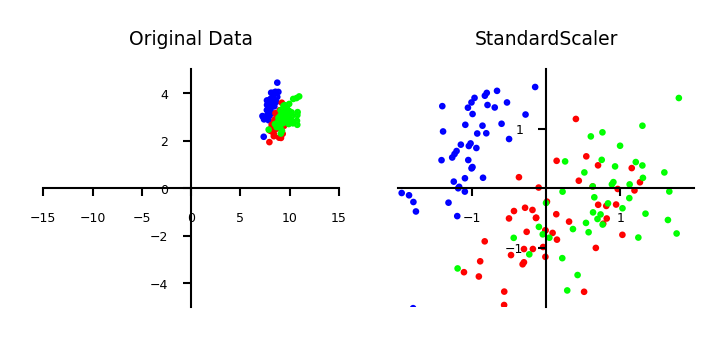
\includegraphics[width=.8\textwidth,keepaspectratio]{images/pre-processing/scaling_1.png}
    \end{figure}
\end{frame}


\begin{frame}{Why do we need scaling?}
    \begin{itemize}
        \item KNN: Distances depend mainly on feature with larger values
        \item SVMs: (kernelized) dot products are also based on distances
        \item Linear model: Feature scale affects regularization
        \begin{itemize}
            \item Weights have similar scales, more interpretable
        \end{itemize}
    \end{itemize}

    \begin{figure}
        \centering
        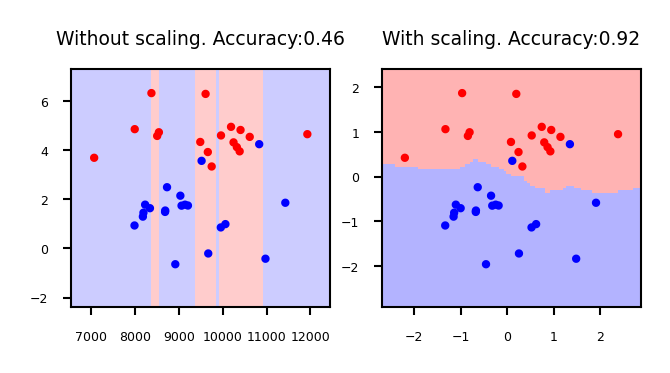
\includegraphics[width=.8\textwidth,keepaspectratio]{images/pre-processing/scaling_2.png}
    \end{figure}
\end{frame}


\begin{frame}{Standard scaling (standardization)}
    \begin{itemize}
        \item Generally most useful, assumes data is more or less normally distributed
        \item Per feature, subtract the mean value $\mu$, scale by standard deviation $\sigma$
        \item New feature has $\mu = 0$ and $\sigma = 1$, values can still be arbitrarily large
    \end{itemize}

    \[
        \mathbf{x_{new}} = \frac{\mathbf{x} - \mu}{\sigma}
    \]

    \begin{figure}
        \centering
        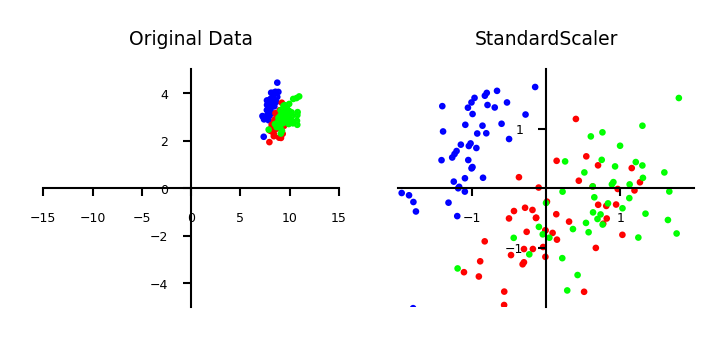
\includegraphics[width=0.8\textwidth,keepaspectratio]{images/pre-processing/scaling_3.png}
    \end{figure}
\end{frame}


\begin{frame}{Min-max scaling}
    \begin{itemize}
        \item Scales all features between a given \textit{min} and \textit{max} value (e.g. 0 and 1)
        \item Makes sense if min/max values have meaning in your data
        \item Sensitive to outliers
    \end{itemize}

    \[
        \mathbf{x_{new}} = \frac{\mathbf{x} - x_{\text{min}}}{x_{\text{max}} - x_{\text{min}}} \cdot (max - min) + min
    \]

    \begin{figure}
        \centering
        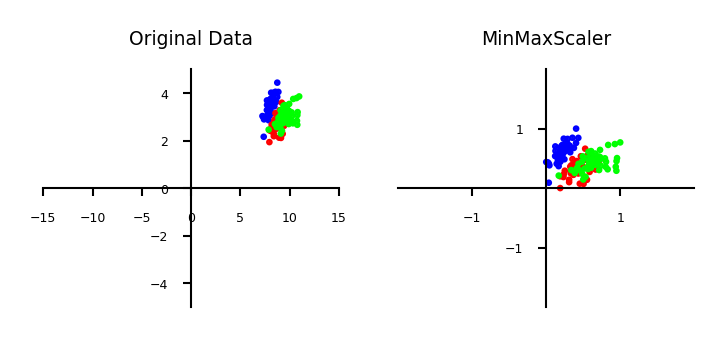
\includegraphics[width=0.8\textwidth,keepaspectratio]{images/pre-processing/scaling_4.png}
    \end{figure}
\end{frame}



\begin{frame}{Robust scaling}
    \begin{itemize}
        \item Subtracts the median, scales between quantiles $q_{25}$ and $q_{75}$
        \item New feature has median 0, $q_{25} = -1$ and $q_{75} = 1$
        \item Similar to standard scaler, but ignores outliers
    \end{itemize}

    \begin{figure}
        \centering
        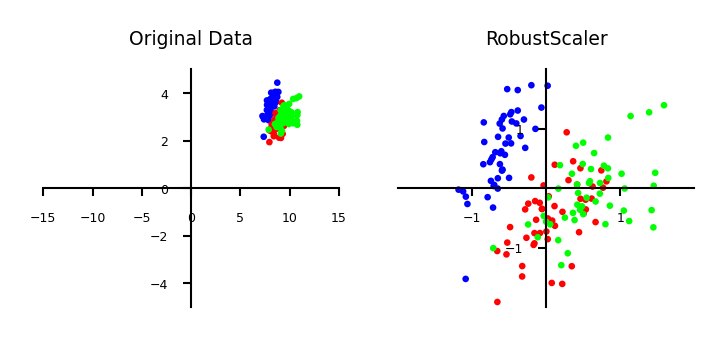
\includegraphics[width=0.8\textwidth,keepaspectratio]{images/pre-processing/scaling_5.png}
    \end{figure}
\end{frame}


\begin{frame}{Normalization}
    \begin{itemize}
        \item Makes sure that feature values of each point (each row) sum up to 1 (L1 norm)
        \begin{itemize}
            \item Useful for count data (e.g. word counts in documents)
        \end{itemize}
        \item Can also be used with L2 norm (sum of squares is 1)
        \begin{itemize}
            \item Useful when computing distances in high dimensions
            \item Normalized Euclidean distance is equivalent to cosine similarity
        \end{itemize}
    \end{itemize}

    \begin{figure}
        \centering
        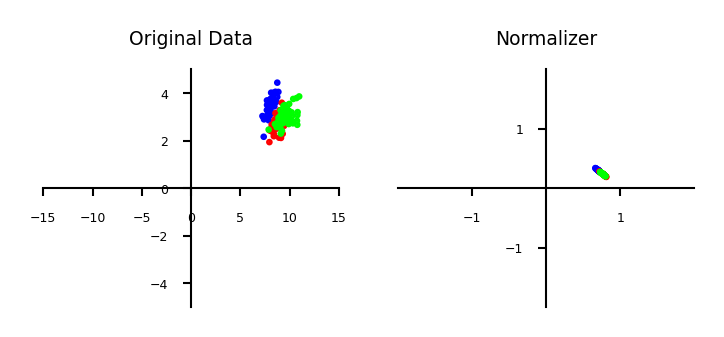
\includegraphics[width=0.8\textwidth,keepaspectratio]{images/pre-processing/scaling_6.png}
    \end{figure}
\end{frame}


\begin{frame}{Maximum Absolute scaler}
    \begin{itemize}
        \item For sparse data (many features, but few are non-zero)
        \begin{itemize}
            \item Maintain sparseness (efficient storage)
        \end{itemize}
        \item Scales all values so that maximum absolute value is 1
        \item Similar to Min-Max scaling without changing 0 values
    \end{itemize}

    \begin{figure}
        \centering
        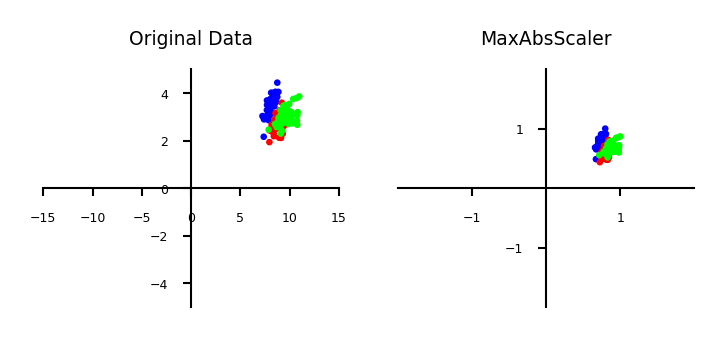
\includegraphics[width=0.8\textwidth,keepaspectratio]{images/pre-processing/scaling_7.png}
    \end{figure}
\end{frame}
